\documentclass{article}
\usepackage[english,russian]{babel}
\usepackage[utf8]{inputenc}
\usepackage{indentfirst}
\usepackage{graphicx}
\usepackage{float}
\usepackage[margin=2cm]{geometry}
\usepackage{hyperref}
\usepackage{forest}
\definecolor{folderbg}{RGB}{124,166,198}
\definecolor{folderborder}{RGB}{110,144,169}

\def\Size{4pt}
\tikzset{
  folder/.pic={
    \filldraw[draw=folderborder,top color=folderbg!50,bottom color=folderbg]
      (-1.05*\Size,0.2\Size+5pt) rectangle ++(.75*\Size,-0.2\Size-5pt);  
    \filldraw[draw=folderborder,top color=folderbg!50,bottom color=folderbg]
      (-1.15*\Size,-\Size) rectangle (1.15*\Size,\Size);
  }
}


\begin{document}
    \begin{titlepage}
        \begin{center}
            ГУАП
            \vspace{0.25cm}

            КАФЕДРА №51
        \end{center}

        \begin{flushleft}

            КУРСОВАЯ РАБОТА (ПРОЕКТ)

            ЗАЩИЩЕН С ОЦЕНКОЙ

            ПРЕПОДАВАТЕЛЬ


            \vspace{0.5cm}
            
            доцент, канд.техн.наук \hspace{10.5cm} Линский Е.М.

            $\rule{5cm}{0.15mm}$ \hfill $\rule{2.2cm}{0.15mm}$  \hfill $\rule{3.25cm}{0.15mm}$

            должность, уч. степень, звание \hfill подпись, дата \hfill инициалы, фамилия
        \end{flushleft}

		\vspace{2cm}

        \begin{center}
            ПОЯСНИТЕЛЬНАЯ ЗАПИСКА\\
			К КУРСОВОЙ РАБОТЕ (ПРОЕКТУ)


            \vspace{1cm}
			
			Почтовый сервис ZenMail

            \vspace{1cm}

            по курсу: ТЕХНОЛОГИИ ПРОГРАММИРОВАНИЯ {\MakeUppercase{\romannumeral 2}}
        \end{center}

        \vspace{6cm}

        \begin{flushleft}
            РАБОТУ ВЫПОЛНИЛИ \hspace{10.55cm} Щипило А.М.\\
            \hspace{14.25cm} Заболотный А.В.\\
    		\hspace{15cm} Костин С.О.

            СТУДЕНТЫ ГР. № 5511 \hfill $\rule{2.2cm}{0.15mm}$  \hfill $\rule{3.25cm}{0.15mm}$

            \hspace{7.8cm} подпись, дата \hfill инициалы, фамилия
        \end{flushleft}

        \vspace{3cm}
        \begin{center}
            Санкт-Петербург 2017
        \end{center}
    \end{titlepage}
        
\newpage
\tableofcontents
\newpage

\section{Функциональная спецификация}
\subsection{Цель}
В качестве основной цели данной курсовой работы была поставлена разработка почтового сервиса с выделенной базой данных, почтовым сервером и функционально полным веб-приложением, позволяющим принимать и отправлять письма зарегистрированным пользователям. \\

Следовательно, в данном случае необходимо было заняться многими направлениями разработки, и разбить большой объем работ над веб-приложением. Так сформировалась команда из трех человек: Андрей Щипило, Артем Заболотный и Сергей Костин. \\

Тогда весь объем работы разбивается на три главных компонента: 
\begin{itemize}
	\item \textbf{Интерактивная часть веб-приложения} –- интерактивная оболочка, созданная при помощи фреймворка Angular 2+. (далее frontend)

	\item \textbf{Программно-аппаратная часть веб-приложения} –- программа на фреймворке Spring с архитектурой REST, управляющая данными с frontend. (далее backend)

	\item \textbf{Почтовый сервер с базой данных} –- сервер, отвечающий за отправку, прием и хранение писем. (далее mailserver)
\end{itemize}


\textbf{Frontend}: это интерфейс взаимодействия между пользователем и программно-аппаратной частью веб-приложения, использующий веб-технологии для обработки информации полученной от пользователя на клиенте или отправляя информацию на \emph{Backend}, предоставляя пользователю полный контроль над своим почтовым ящиком, включая регистрации, аутентификацию, а также просмотр и отправку сообщений. \\

\textbf{Backend}: это программа, исполняющаяся на предполагаемом сервере, которая обрабатывает информацию и отвечает на запросы от \emph{Frontend}, выполняя необходимые действия (прим. добавление нового пользователя в базу данных). Для улучшения опыта использования веб-приложения сервер должен своевременно и быстро обрабатывать запросы от нескольких пользователей одновременно. Именно с этого приложения происходит запросы почтовому серверу на отправку и чтение писем, по протоколам IMAP, POP3 и SMTP. \\

\textbf{Mail Server}: это специально настроенный сервер, размещенный на сервере, который может быть использован большую часть времени (прим. облачное хранилище). На машине в облаке установлены и конфигурированы программы для отправки и принятия писем, проверки писем на спам, вирусы, а также для аутентификации и шифрования соединений. Причем именно на этом сервер хранится и база данных, с которой активно взаимодействует \emph{Frontend} часть веб-приложения. \\

\subsection{Основные функции}

Основные функции программы:

\begin{itemize}
  \item Возможность подключения к почтовому серверу не только с реализованного в курсовой работе веб-приложения
  \item Регистрация новых пользователей через форму.
  \item Вход в почтовый ящик по логину и паролю.
  \item Просмотр пришедших писем.
  \item Поиск по письмам.
  \item Создание нового письма с базовым редактированием.
\end{itemize}

\subsection{Технологии}

\begin{table}[]
\centering
\begin{tabular}{|l|l|}
\hline
\multicolumn{1}{|c|}{\textbf{Component}} & \multicolumn{1}{c|}{\textbf{Technology}} \\ \hline
Frontend                                 & Angular 4+ and Covalent                  \\
Backend (REST)                           & SpringBoot (Java)                        \\
Security                                 & Token                                    \\
Persistence                              & JPA (Using Spring Data)                  \\
Client Build Tools                       & angular-cli, Webpack, npm                \\
Server Build Tools                       & Maven (Java)                             \\ \hline
\end{tabular}
\caption{Стэк технологий}
\label{my-label}
\end{table}

Кроме основного стэка технологий будут использоваться дополнительные сторонние разработки и программы для обеспечения быстроты, удобства разработки и использования, а также общей безопасности системы: \\

\begin{itemize}
\item Ubuntu Server 16.04 LTS
\item Postfix, MTA
\item Dovecot
\item MySQL
\item Rspamd
\item Amazon EC2
\end{itemize}

\subsection{Команда}
Так как существовали установленные сроки сдачи курсовой работы, необходимо было распределить курс работ равномерно между всеми участниками проекта, чтобы максимизировать участие каждого из участников в проекте и минимизировать время затраченное в ожидании результатов одного из участников.
В конечном итоге было предложено такое распределение по обязанностям:
\begin{itemize}
\item Щипило Андрей: занимается общей архитектурой веб-приложения SpringFramework, правильной инициализацией процессов приложения через SpringBoot и Maven, графическим и пользовательским представлением веб-приложения, используя возможности Angular 4, менеджментом проекта, а также настройкой и поддержанием почтового сервера в облачном хранилище.

\item Костин Сергей: занимается обработкой данных почтового сервера и веб-приложения, используя MariaDB и Spring Data, представлением данных в программе, а отвечает за безопасную аутентификацию пользователей через токены и фильтры безопасности системы, используя Spring Security и защищённые протоколы связи.

\item Заболотный Артем: занимается связью между программной и графической частями приложения, используя нативный для Angular 4 язык программирования TypeScript,  из Spring Security, является менеджером глобального тестирования веб-приложения, а также за защищенную связь через почтовые протоколы IMAPS и SMTPS, позволяющую безопасно связать программную часть веб-приложения и почтовый сервер.
\end{itemize}
\newpage

\section{Особенности реализации}
Для более подробного описания, а также документации лучше всего обратиться на официальную страницу приложения на сервисе github.\\
\url{https://github.com/ProjectZenMail/zenmail}

\begin{figure}[H]
        \begin{flushleft}
            \centerline{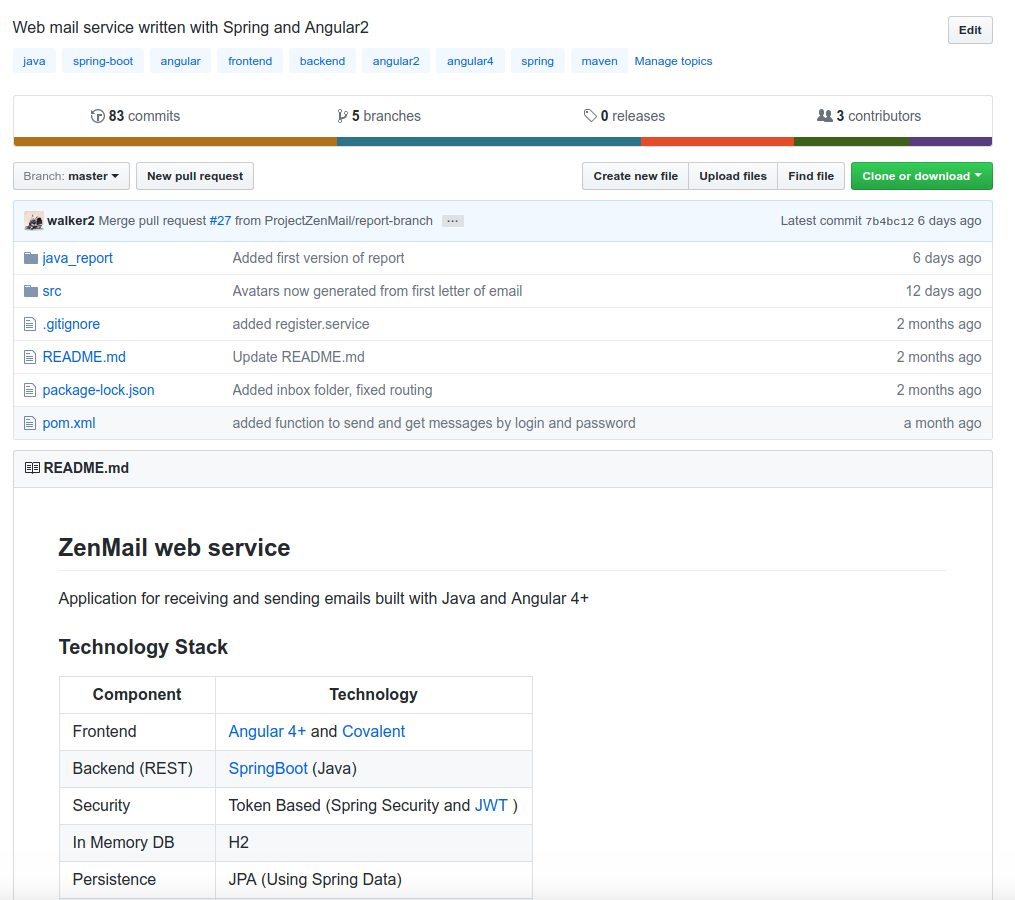
\includegraphics[scale=0.6]{githubpage.png}}
            \caption{Страница проекта на сервисе GitHub}
        \end{flushleft}
\end{figure}

\subsection{Backend}
Для разработки такого, достаточно масштабного, проекта необходимо было найти некий фреймворк, который облегчил поставленную задачу. В качестве такого фремворка был выбран самый популярный на данный момент -- Spring Framework, который позволяет упростить настройку и конфигурацию сервера и обеспечить все необходимые компоненты для разработки программной части полноценного веб-приложения. \\

Так как SpringFramework -- это популярный комплексный фреймфорк для разработки веб-приложений, то у него большое количество настроек. Для упрощения запуска и отладки нашего веб-приложения используется модуль \textbf{SpringBoot}: с помощью аннотации @SpringBootApplication для нашего запускающего класса SpringBoot освобождает нас от слишком глубокой настройки приложения и позволяет собирать, размещать и запускать приложение с помощью одной команды -- springboot:run. Данная команда за нас компилирует код, запускает движок сервлетов Tomcat, создает соответствия для RESTapi и загружает необходимые сервлеты. \\

Но у нас все также остается возможность модифицировать необходимые конфигурационные переменные через изменение файла application.properties, так например мы можем задать адрес нашей базы данных, указать порт для запуска сервера или отключить дополнительные модули для тестирования.  \\

Кроме Spring'a были использованы библиотеки, облегчающие некоторые аспекты. Например, для уменьшения кода при написании приватных полей классов модели был использована библиотека \textbf{Lombok}. Так же для отправки и принятия сообщений была использована библиотека \textbf{javax.Mail}. Для сборки и загрузки модулей, а также для тестирования и генерации jar файла был использован Maven. \\

Для обеспечения безопасности аутентификации был использован модуль SpringFramework -- \textbf{Spring Security}. А именно были созданы фильтры, запрещающие доступ к скрытым данным через запросы, создана аутентификация на токенах и фильтры Spring Security для проверки подлинности токенов пользователей. Диаграмма работы аутентификации через токены приведена ниже: 

\begin{figure}[H]
        \begin{flushleft}
            \centerline{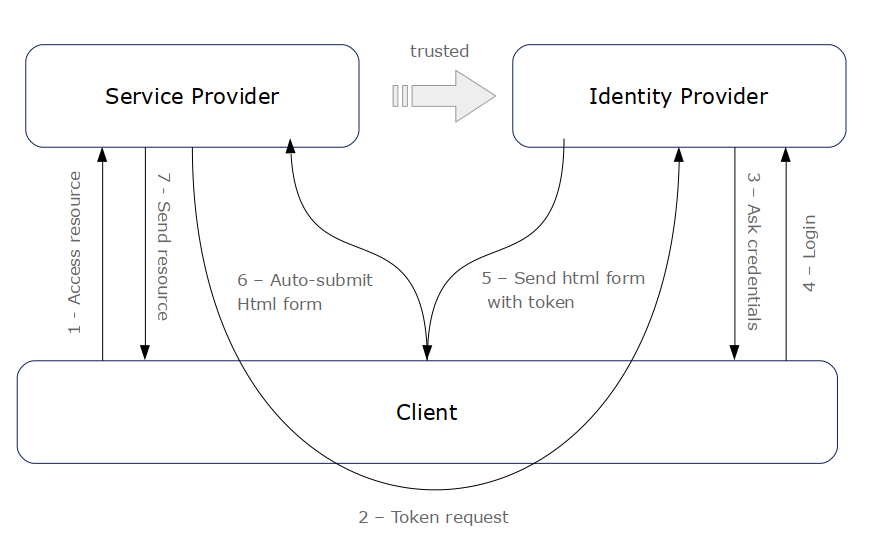
\includegraphics[scale=0.6]{tokenauth.png}}
            \caption{Аутентификация через токены}
        \end{flushleft}
\end{figure}

Для простоты и элегантности кода было решено использовать \textbf{JPA} из SpringFramework, чтобы создать Repository слой, предназначенный для CRUD функций взаимодействия с базой данных. \\

Из-за большого количества модульных компонентов необходимо было упростить сборку и тестирование отдельных компонентов. Для данной задачи был использован \textbf{Apache Maven} -- фреймворк для автоматизации сборки проектов. С его помощью можно было не заботится о скачивании и установки новых модулей, так как Maven берет их со своих серверов и подключает к приложению. Для запуска всего модуля Backend необходимо было ввести лишь одну команду -- mvn clean install, а затем запустить сгенерированный jar файл с помощью java -jar ./target/zenmail-0.0.1.jar. 

Некоторые из важных методов Backend'a:
\begin{enumerate}
\item MainController -- класс, который возвращает index.html, когда требуется mapping '/'. Нужен, чтобы выдавать экран загрузке при запуске веб-приложения.

\item UserService -- класс, который огранизует доступ в свои репозитории (данные из базы данных) и предоставляет возможность работы с ними.
	\begin{itemize}
	\item addNewUser(User user) -- добавляет нового пользователя в репозитории UserRepository
	\item getLoggedInUser() -- возвращает всю информацию, в виде класса User, о залогиненном пользователе.
	\end{itemize}
	
\item UserController -- класс, который использует класс UserService, для возвращения необходимых значений, связывая вызовы GET и POST по пути /user.
	\begin{itemize}
	\item getUserInformation() -- вызывает getLoggedInUser() класса UserService и возвращает результат в виде UserResponse, который хранит в себе информацию о пользователе в виде класса User.
	\item getLoggedInUser() -- возвращает всю информацию, ввиде класса User, о залогиненном пользователе.
	\end{itemize}
	
\item MessagesService -- класс, который хранит необходимые сведения и методы для отправки писем
	\begin{itemize}
	\item getMessages(User user) -- возвращает все доступные сообщения конкретного пользователя в качестве вектора IMAPMessage.
	\item sendMessage(String addressTo, String subject, String text, User user) -- отправляет сообщение по указанному адресу, с указанной темой, текстом от определенного пользователя.
	\end{itemize}
	
\item MessagesController -- класс, который использует класс MessagesService, для возвращения необходимых значений, связывай вызовы GET и POST по пути /messages.
	\begin{itemize}
	\item getUserInformation() -- вызывает getMessages() класса MessagesService и возвращает результат в виде MessagesResponse, который хранит в себе вектор всех сообщений.
	\item sendMessage() -- возвращает всю информацию, ввиде класса User, о залогиненном пользователе.
	\end{itemize}
\end{enumerate}

\subsubsection{Тестирование}
Для тестирования был использованы библиотеки \textbf{Spring Test} и \textbf{JUnit 4}. Были написаны тестирующие программы для всех основных задач api, а именно регистрацию, авторизацию, принятие и отправку сообщений. Для создания имитационных объектов (mock objects) был использован фреймворк \textbf{Mockito}.

\subsection{Mail Server}
Для корректной работы приложения, а именно для базовой авторизации, необходимо было предоставить место для хранения данных пользователей. И, так как почтовый сервер необходимо было разместить на компьютере с открытыми необходимыми портами для различных почтовых протоколов. Было решено использовать реляционную базу данных на основе системы управления базами данных \textbf{MariaDB}. \\

Схема базы данных mail приведена ниже:
\begin{figure}[H]
        \begin{flushleft}        \centerline{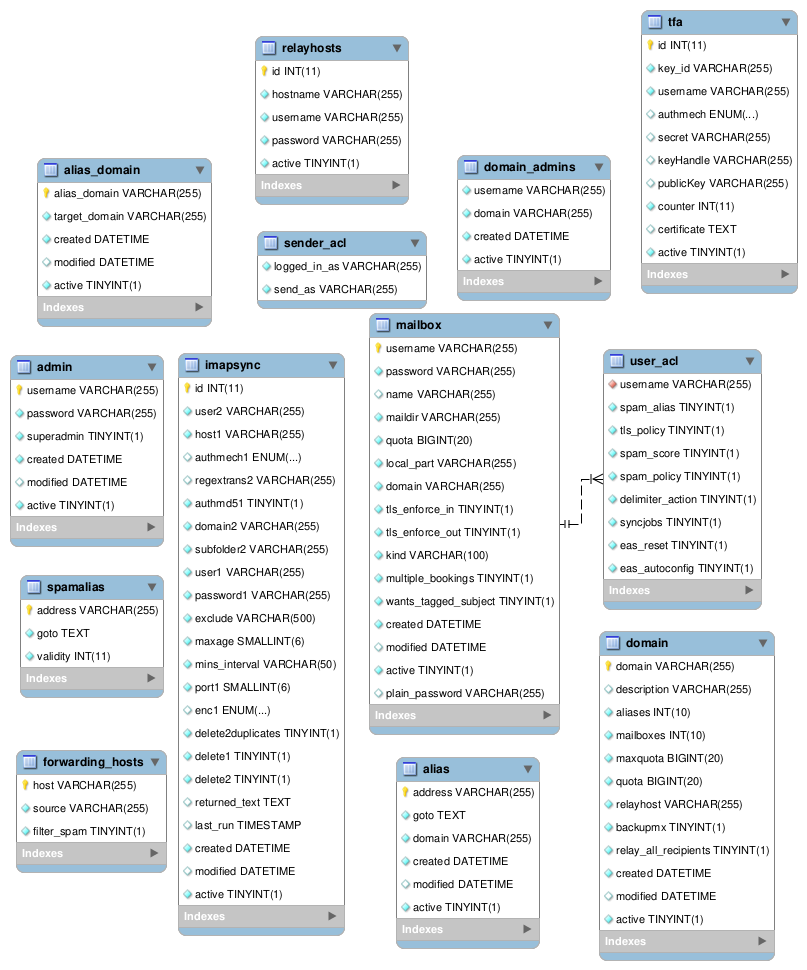
\includegraphics[scale=0.4]{scheme2.png}}
        \caption{Взаимодействие составляющих проекта}
        \end{flushleft}
\end{figure}

Основными таблицами, с которыми осуществляет взаимодействие программа являются \emph{mailbox} и \emph{user}, предоставляющие всю необходимую информацию о пользователе. \\

Остальные же таблицы необходимы для работы программ, отвечающих за работу почтового сервера.

Одной из главных таких программ является \textbf{Dovecot} -- это свободный IMAP- и POP3-сервер с упором на безопасность. Из-за возможности гибкой настройки программы с помощью конфигурационных файлов
можно кардинально поменять принцип работы программы. В проекте используется IMAP аутентификация пользователя, так как она требует меньше дополнительных затрат ресурсов на создание копии ящика пользователя на клиенте, и просто каждый раз забирает почту по TCP протоколу, что, конечно, накладывает некие ограничения на скорость работы. \\

Именно с этой программой связывается Backend часть приложения и запрашивает определенную информацию (напр. входящие письма), авторизировавшись по логину и паролю. Dovecot настроен так, чтобы хранить письма пользователей в виртуальных папках системы, в которой он установлен. Это, а также каким способом авторизоваться программе, по какой таблице определять письма и прочее описывается в конфигурационных файлах Dovecot. \\

Второй программой является агент передачи почты (MTA) \textbf{Postfix}. Как можно понять из названия, именно через эту программу отправляются письма через протокол SMTP. Для данной программы тоже существует множество настроек, которые задаются в конфигурационных файлах. \\

Также установлены и другие программы, необходимые для фильтрования спама и осуществления передачи через TLS протоколы (напр. rspamd). \\

Так как все эти программы требуют портов, которые обычно закрыты на роутерах обычных компьютеров, и сама суть сервера подразумевает постоянную работу всех этих приложений, то было принято решение использовать облачные вычисления от Amazon Web Services -- $EC^2$. 
Вся настройка сервера происходила через сетевой протокол SSH, который позволяет подключаться к операционной системе удаленных систем с помощью приватного и публичного ключа.  \\

Так как требовалось большое количество испытаний прежде чем был бы найден оптимальный вариант настройки конфигурационных файлов приложений, а некоторые из них достаточно сложно найти в установленной системе и при изменении одной строчки конфигурационного файла могла лечь вся программа, то было принято решение использовать \textbf{docker}. Docker позволяет автоматизировать развертывание и управление приложениями в виртуализированной среде. Так как нам нужно было использовать много контейнеров для различных приложений, то был использован \textbf{Docker Compose}, который позволяет запускать мультиконтейнерные приложения через конфигурационный файл и команду docker-compose up. \\

\newpage
Ниже представлена структура папок docker

\begin{forest}
      for tree={
        font=\ttfamily,
        grow'=0,
        child anchor=west,
        parent anchor=south,
        anchor=west,
        calign=first,
        inner xsep=7pt,
        edge path={
          \noexpand\path [draw, \forestoption{edge}]
          (!u.south west) +(7.5pt,0) |- (.child anchor) pic {folder} \forestoption{edge label};
        },
        % style for your file node 
        file/.style={edge path={\noexpand\path [draw, \forestoption{edge}]
          (!u.south west) +(7.5pt,0) |- (.child anchor) \forestoption{edge label};},
          inner xsep=2pt,font=\small\ttfamily
                     },
        before typesetting nodes={
          if n=1
            {insert before={[,phantom]}}
            {}
        },
        fit=band,
        before computing xy={l=15pt},
      }  
    [mailserver
      [data
        [Dockerfiles
        	[acme
        	]
        	[clamd
        	]
        	[dovecot
        		[Dockerfile,file]
        	]
        	[mysql
        	]
        	[postfix
        		[Dockerfile,file]
        	]
        	[redis
        	]
        	[rspamd
        	]
        ]
        [assets
        ]
        [conf
        	[dovecot
        		[dovecot.conf,file]
        	]
        	[mysql
        		[my.cnf,file]
        	]
        	[postfix
        		[main.cf,file]
        		[master.cf,file]
        	]
        ]
      ]
      [docker-compose.yml,file
      ]
      [mailserver.conf,file
      ]
    ]
 \end{forest}
 
\subsection{Frontend}
Для того, чтобы конечный пользователь мог удобно взаимодействовать с описанным выше почтовым сервером, необходимо было создать оболочку веб-приложения. \\

Для этой цели был использован фреймворк веб-приложений \textbf{Angular2+}, который позволяет упростить создание интерактивных сайтов, при этом добавляя множество функций. Одна из главных -- это возможность написания на строго типизированном языке программирования \textbf{TypeScript}, \\

Ниже приведена схема архитектуры фреймворка Angular2+
\begin{figure}[H]
        \begin{flushleft}        \centerline{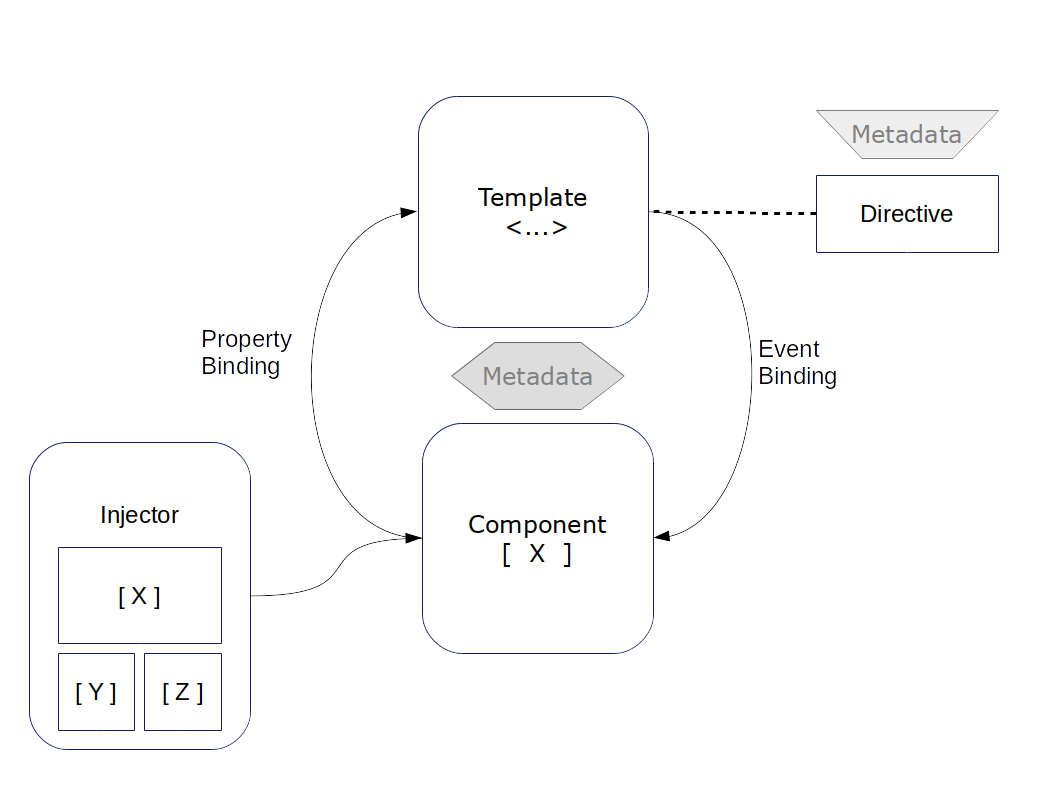
\includegraphics[scale=0.45]{angulararch.png}}
        \caption{Архитектура фреймворка Angular2+}
        \end{flushleft}
\end{figure}

Для упрощения графическо-дизайнерской стороны был использован модуль angular-material, который предоставляет набор различных элементов для придания веб-приложению вида material-design. 

Для сборки веб-приложения был использован модуль \textbf{angular-cli}.
Из-за большого количества остальных модулей, от которых зависят многие вышеописанные модули, был использован менеджер пакетов - \textbf{npm}, который скачивает и подсоединяет модули к проекту.

\section{Описание архитектуры проекта}
Проект, как говорилось раньше, можно разделить на три главные составляющие: Frontend, Backend и MailServer. В общем виде Frontend посылает запрос Backend'у, и в большинстве случаев Backend посылает запрос базе, получает ответ, обрабатывает и отсылает на Frontend. \\
Общее взаимодействие между основными компонентами проекта можно наблюдать на схеме ниже. 

\begin{figure}[H]
        \begin{flushleft}        \centerline{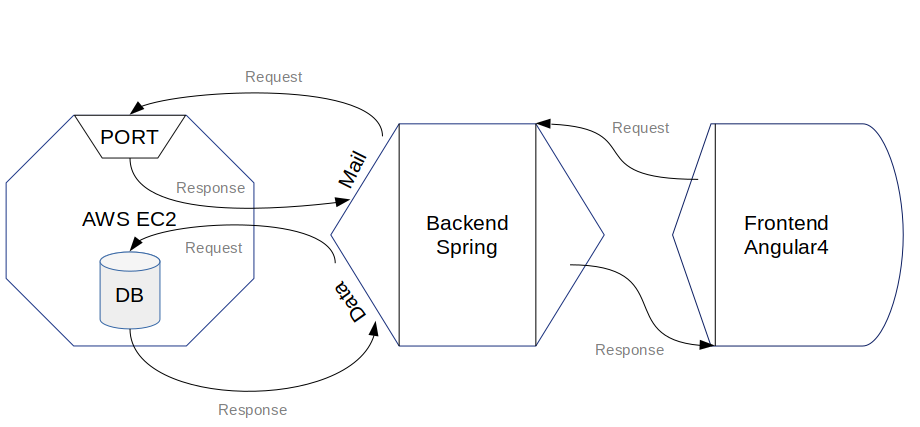
\includegraphics[scale=0.6]{basicscheme.png}}
        \caption{Взаимодействие составляющих проекта}
        \end{flushleft}
\end{figure}

Веб-приложение организованно с помощью паттерна проектирования Model-View-Control (MVC), где моделями являются различные внутренние представления (напр. User, у которого есть имя, директории, логин и т.д.), control -- это сервисы и контроллеры для управления моделями (напр. у MessagesController есть метод sendMessage, который отсылает сообщение по IMAP, используя сервис MessagesService), view -- это отображение наших данных (напр. сообщений) с использованием фреймворка Angular 4.

\begin{figure}[H]
        \begin{flushleft}        \centerline{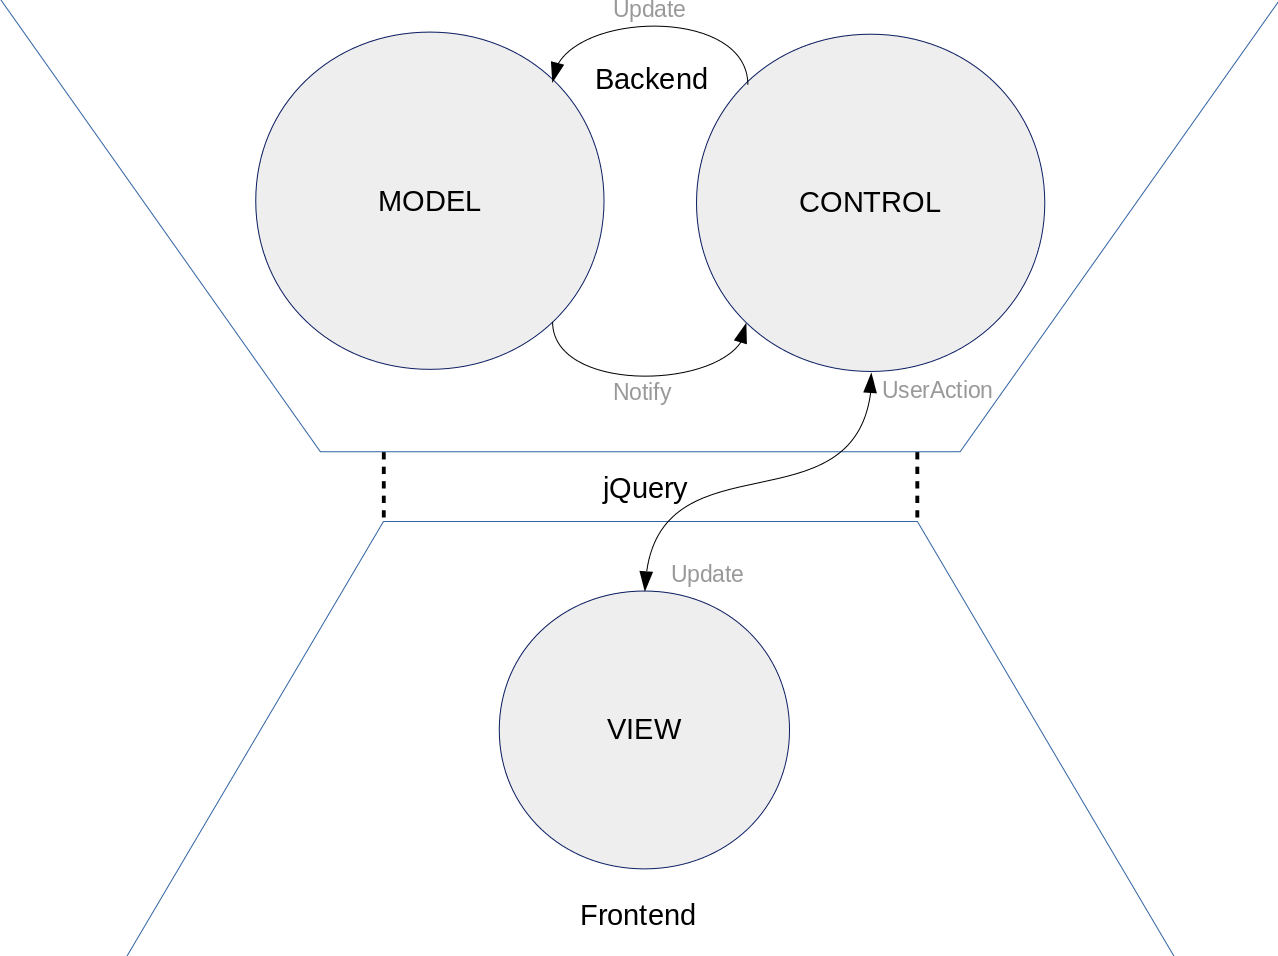
\includegraphics[scale=0.3]{mvc.png}}
        \caption{Взаимодействие составляющих проекта}
        \end{flushleft}
\end{figure}

\section{Руководство пользователя}

\subsection{Авторизация}
После перехода на адрес веб-приложения пользователя перенаправят на страницу авторизации.
\begin{figure}[H]
        \begin{flushleft}
            \centerline{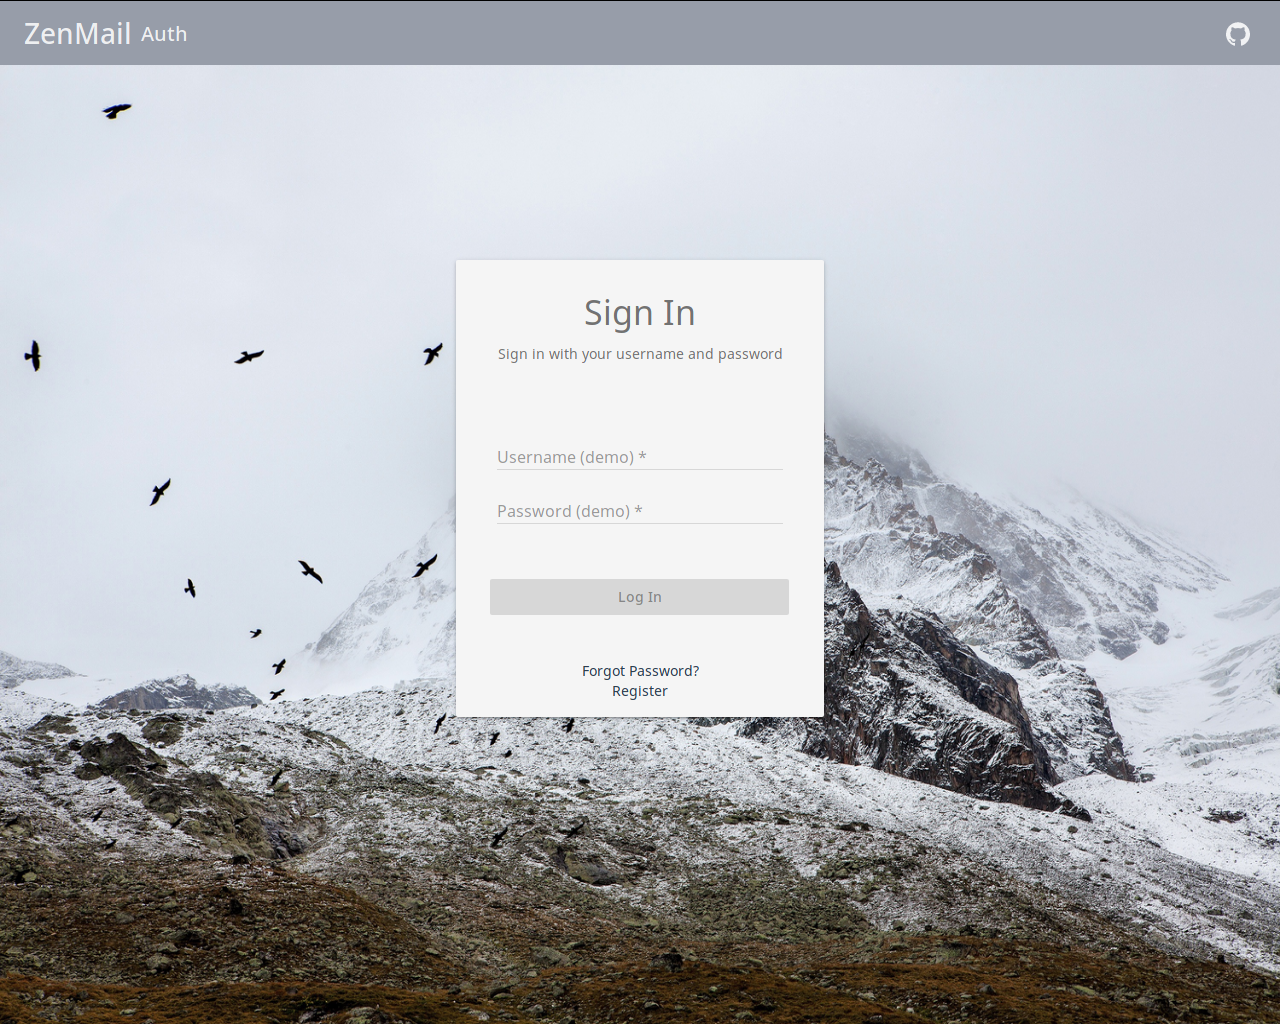
\includegraphics[scale=0.6]{loginscreen.png}}
            \caption{Страница авторизации}
        \end{flushleft}
\end{figure}

Если у пользователя нет действующей почты он может перейти на страницу регистрации, нажав на ссылку Register.

\begin{figure}[H]
        \begin{flushleft}
            \centerline{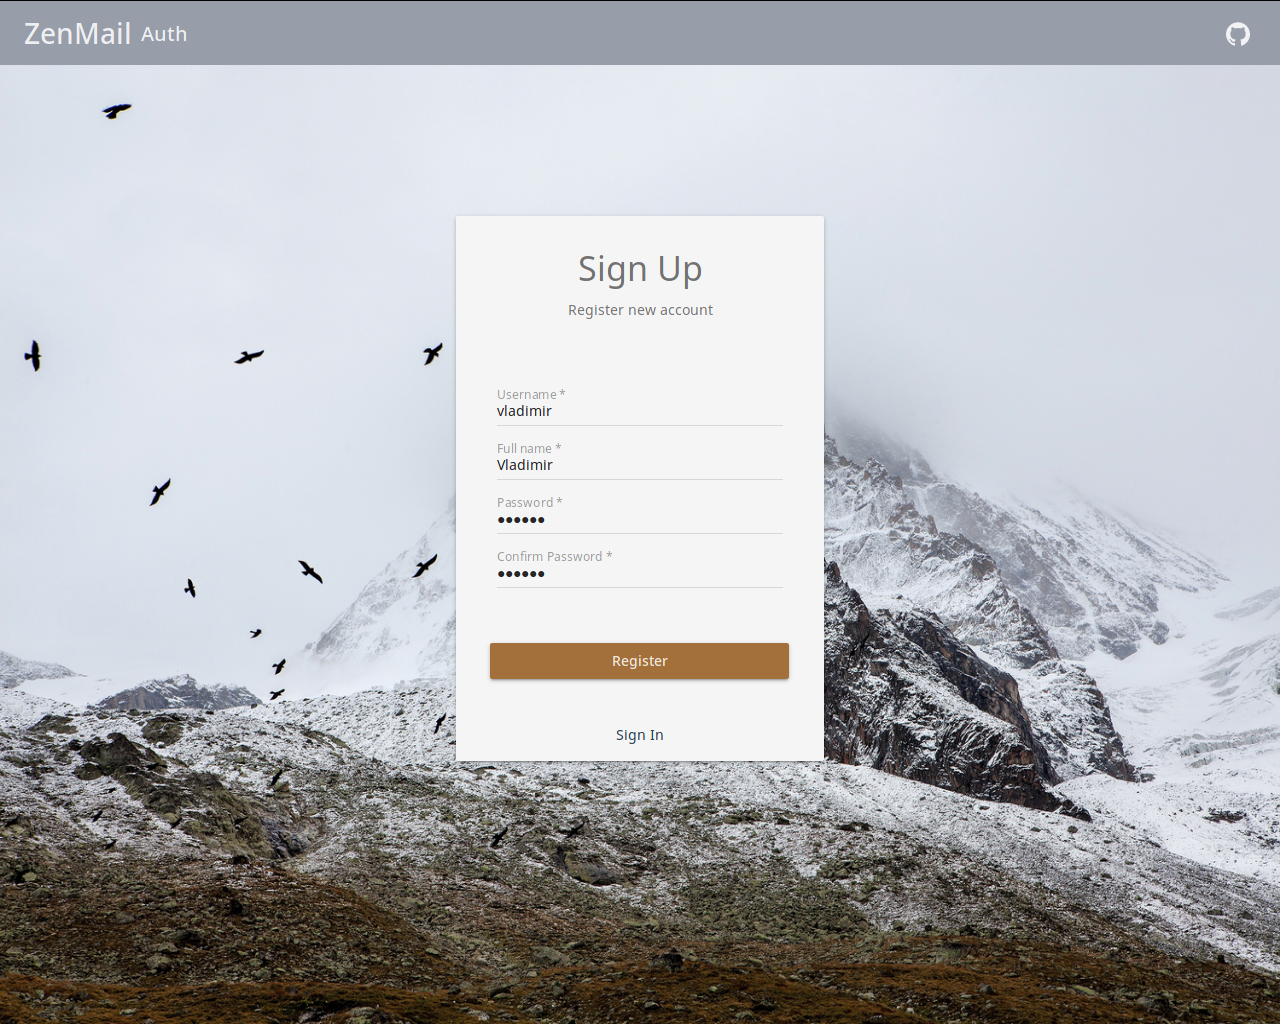
\includegraphics[scale=0.6]{register.png}}
            \caption{Страница регистрации}
        \end{flushleft}
\end{figure}

После верного заполнения всех полей пользователя перенаправит на главную страницу с письмами.
\begin{figure}[H]
        \begin{flushleft}
            \centerline{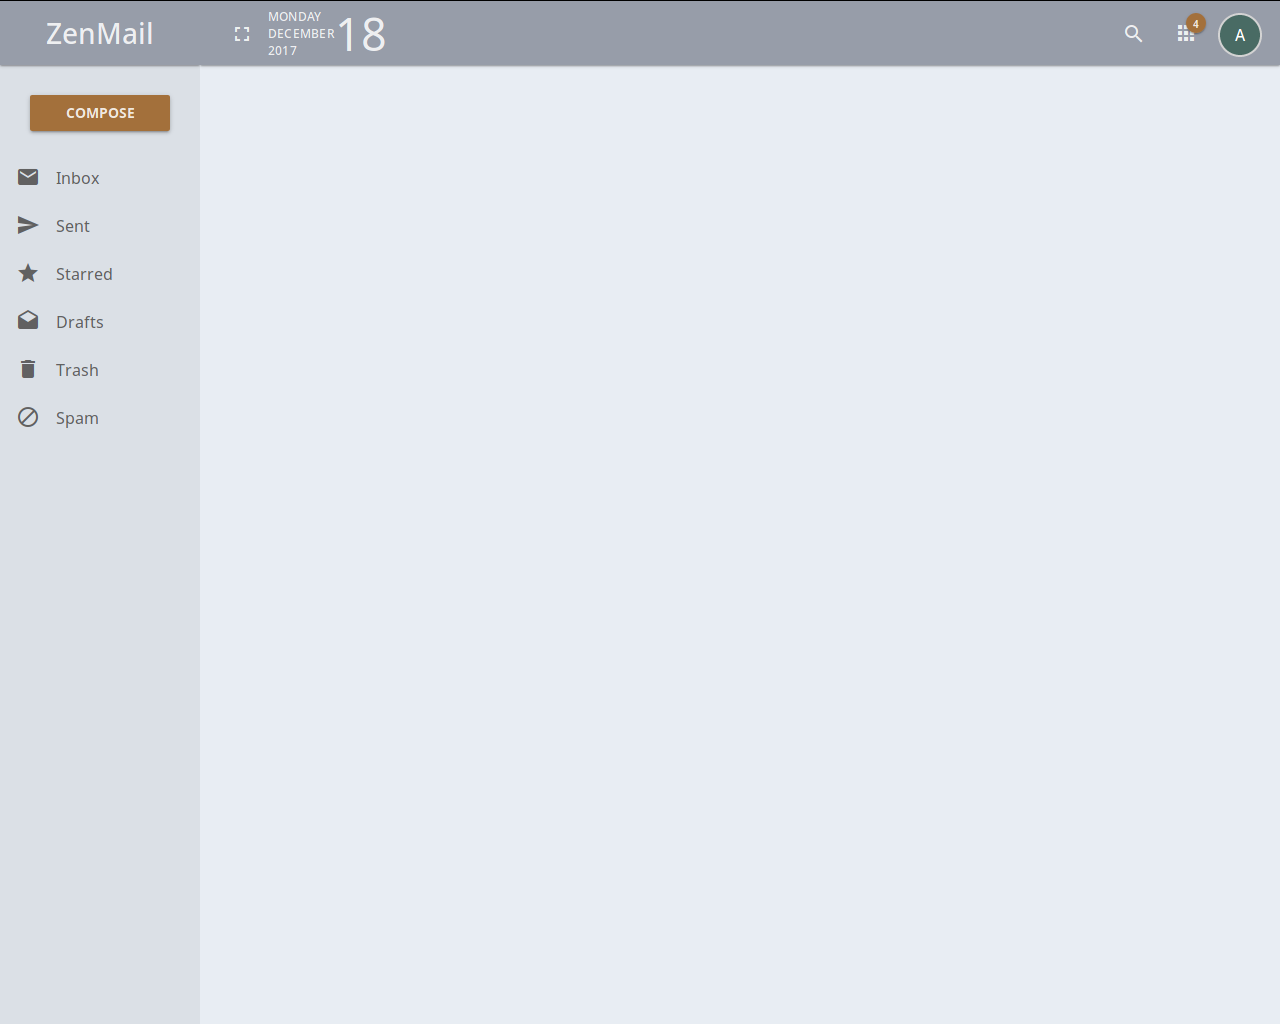
\includegraphics[scale=0.6]{homescreen.png}}
            \caption{Домашняя страница авторизированного аккаунта}
        \end{flushleft}
\end{figure}

После перехода на домашнюю страницу пользователь может управлять своим почтовым аккаунтом. \\

\subsection{Входящие сообщения}
При нажатии на кнопку Inbox открывается страница со всеми входящими сообщениями на данном аккаунте.

\begin{figure}[H]
        \begin{flushleft}
            \centerline{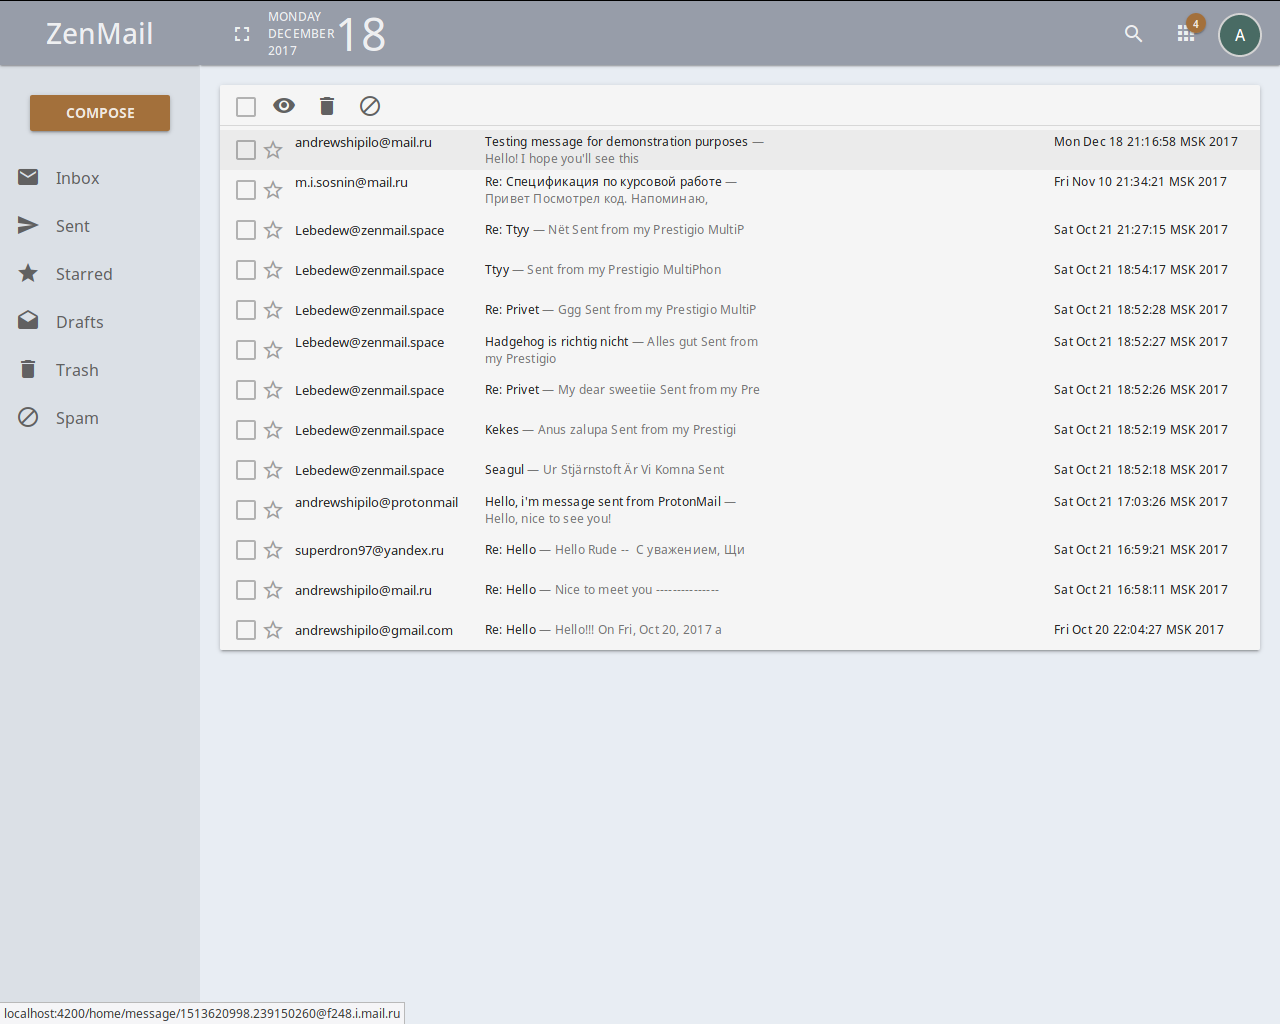
\includegraphics[scale=0.6]{inbox.png}}
            \caption{Входящие сообщения}
        \end{flushleft}
\end{figure}

При нажатии на любое из сообщений мы можем открыть его 

\begin{figure}[H]
        \begin{flushleft}
            \centerline{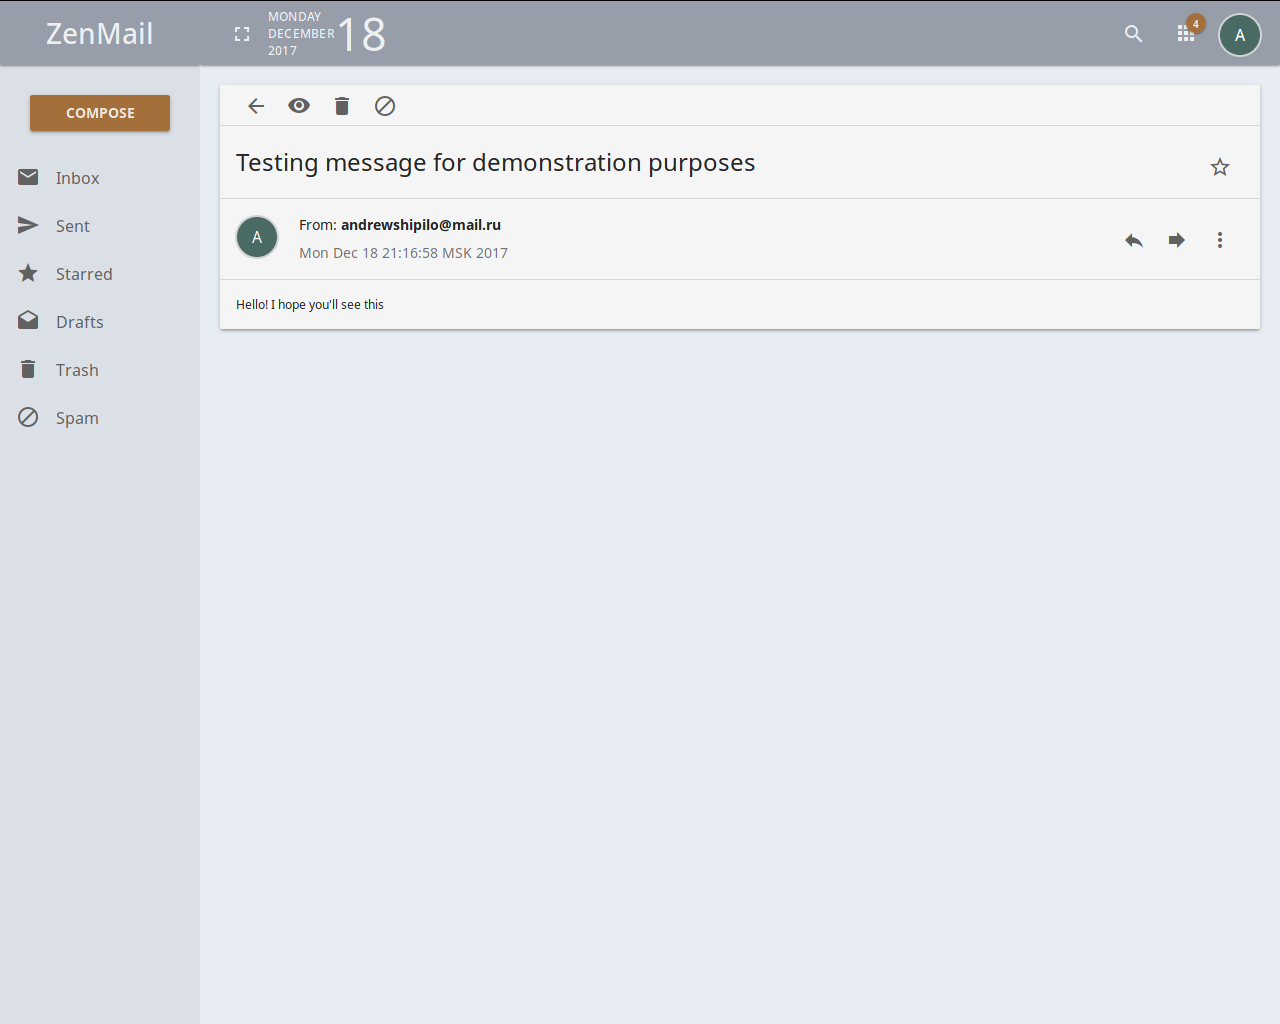
\includegraphics[scale=0.6]{message.png}}
        \caption{Содержимое сообщения}
        \end{flushleft}
\end{figure}

\subsection{Отправка сообщения}
Для того, чтобы отправить сообщение нужно нажать на кнопку COMPOSE, после этого появится форма отправки сообщения, где можно указать получателя, тему и текст сообщения. Эту форму можно закрыть, нажав на крестик в правом углу. Для того, чтобы отправить сообщение необходимо нажать на самолетик.

\begin{figure}[H]
        \begin{flushleft}        \centerline{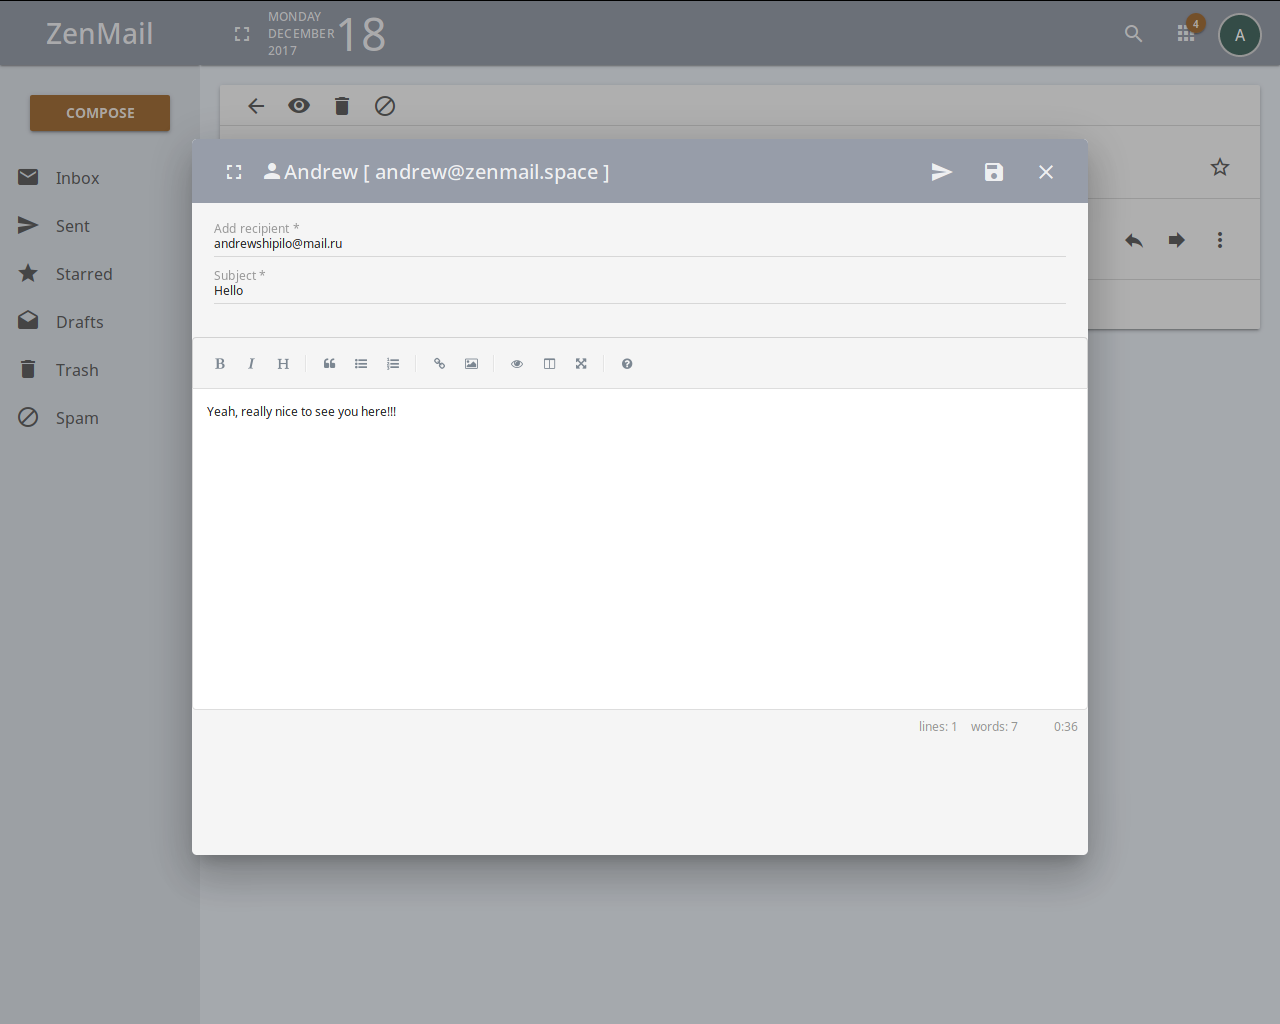
\includegraphics[scale=0.6]{sendmessage.png}}
        \caption{Форма отправки сообщения}
        \end{flushleft}
\end{figure}

При отправке сообщения форма закроется и появится уведомление с результатом отправки сообщения.

\begin{figure}[H]
        \begin{flushleft}        \centerline{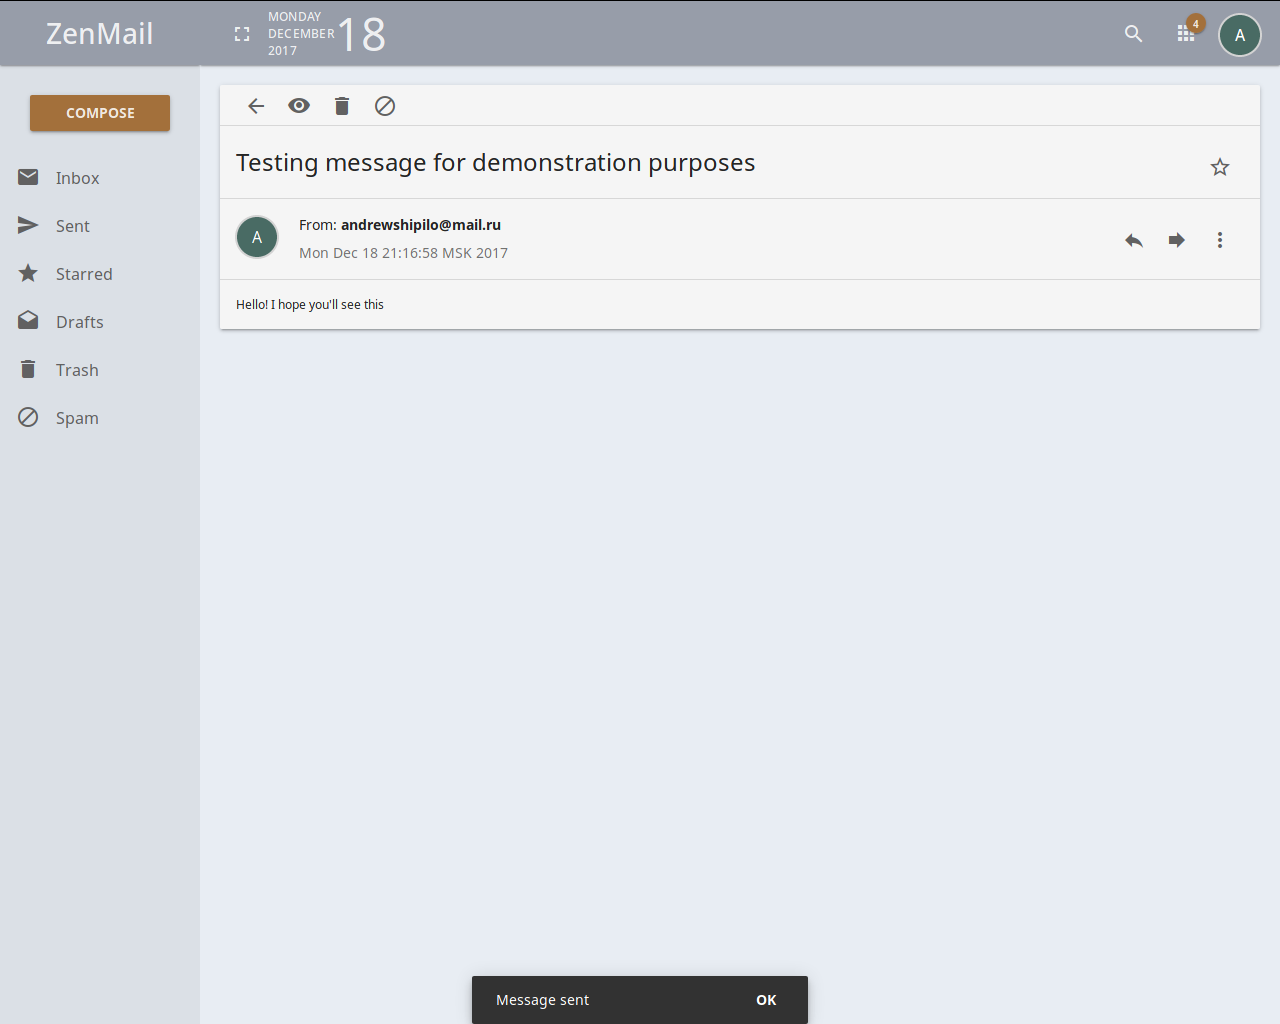
\includegraphics[scale=0.6]{messagesent.png}}
        \caption{Уведомление об отправке сообщения}
        \end{flushleft}
\end{figure}

\newpage


\end{document}